\begin{figure}

\mode
<presentation>

\vspace*{-0.2cm}

\mode
<all>

\vspace*{-0.25cm}

\hspace*{-0.025\columnwidth}
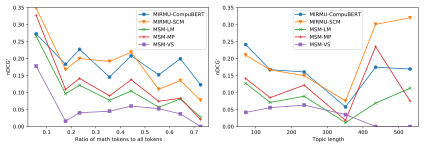
\includegraphics[width=1.025\columnwidth, trim={0 3.9mm 0 0}, clip]{strengths-and-weaknesses}

\mode
<article>

\caption
  [Strengths and weaknesses of six diverse systems]%
  {The accuracies (on the $y$-axis) of six diverse math information retrieval 
   systems for different ratios of math tokens to all tokens in a query (left)
   and for different query lengths (right). \cite[Figure 8]{novotny2021ensembling}}

\mode
<presentation>

\vspace*{-0.2cm}

\caption
  {The accuracies (on the $y$-axis) of six diverse math information retrieval 
   systems for different ratios of math tokens to all tokens in a query (left)
   and for different query lengths (right). -- \textcite[Figure 8]{novotny2021ensembling}}

\mode
<all>

\label{fig:strengths-and-weaknesses}
\end{figure}
